\documentclass[12pt, twoside]{report}
\usepackage[TS1,T1]{fontenc}
\usepackage{lmodern}
\usepackage[utf8]{inputenc}
\usepackage{newunicodechar}
\newcommand*\longs{{\fontencoding{TS1}\selectfont s}}
\newunicodechar{ſ}{\longs}
\usepackage[a4paper,width=150mm,top=25mm,bottom=25mm,bindingoffset=6mm]{geometry}
\usepackage{enumitem}
\usepackage{amsmath}
\usepackage{float}
\usepackage{graphicx}
\usepackage{caption}
\usepackage{subcaption}
\usepackage[backend=bibtex, style=authoryear, maxcitenames=2]{biblatex}
\addbibresource{references.bib}
\usepackage{cleveref} % cleverref has to be loaded after hyperref!
\crefname{lstlisting}{listing}{listings}
\Crefname{lstlisting}{Listing}{Listings}
\usepackage{wrapfig}
\usepackage[colorinlistoftodos]{todonotes} % dont forget to remove
\usepackage{url}
\makeatletter
\g@addto@macro{\UrlBreaks}{\UrlOrds} % linebreaks of urls at - and other
\makeatother

% listings
\usepackage{listings}
\lstset{
	captionpos=b,
	frame=single,
	breaklines=true,
	tabsize=2,
	literate=%
		{Ö}{{\"O}}1
		{Ä}{{\"A}}1
		{Ü}{{\"U}}1
		{ß}{{\ss}}1
		{ü}{{\"u}}1
		{ä}{{\"a}}1
		{ö}{{\"o}}1
		{~}{{\textasciitilde}}1,
	alsoletter={{\"u}}
}
\definecolor{maroon}{rgb}{0.5,0,0}
\definecolor{darkgreen}{rgb}{0,0.5,0}
\lstdefinelanguage{XML}
{
	basicstyle=\ttfamily\footnotesize,
	morestring=[s]{"}{"},
	morecomment=[s]{?}{?},
	morecomment=[s]{!--}{--},
	commentstyle=\color{darkgreen},
	moredelim=[s][\color{black}]{>}{<},
	moredelim=[s][\color{red}]{\ }{=},
	stringstyle=\color{blue},
	identifierstyle=\color{maroon}
}

\usepackage{mdframed}
\newmdtheoremenv{defn}{Definition}[chapter]

\begin{document}

\begin{titlepage}
    \begin{center}
        \vspace*{1cm}
        
        \Huge{\textbf{Extracting recipe ingredients from cookbooks}}
        
        \vspace{1cm}
        
        \Large{by}\\
        \LARGE{Torsten Knauf}
        
        \vspace{1cm}
        
        \Large
        A thesis presented for the degree of\\
        Master of Science
        
        \vspace{1cm}
        
        
\includegraphics[width=0.4\textwidth]{Images/cau-siegel.pdf}
        
        Research Group for Communication Systems\\
        \large{at} \\
        Faculty of Engineering\\
        Christian-Albrechts-Universität zu Kiel\\
        Germany\\
        31.03.2017
    \end{center}
    
    \vspace{1cm}
    
    \LARGE
    \begin{tabbing}
    Supervisor: \= Prof. Dr.-Ing.Norbert Luttenberger\\
    \> Dr.-Ing. Jesper Zedlitz
    \end{tabbing}
\end{titlepage}

\pagenumbering{Roman}
\chapter*{Abstract}
Always do this one last, when knowing the things to praise  yourself for :P

\chapter*{Acknowledgements}
If I don't profit from nice people in these thesis, I have done something horrible wrong. So try to remember most of them here at the end... :)

Arbeitsgruppe, stackoverflow
\tableofcontents

\listoffigures
\begingroup
	\let\clearpage\relax
	\listoftables
\endgroup

\clearpage
\pagenumbering{arabic}  
\chapter{Introduction}
80-120Seiten anpeilen
\section{Problem-Stellung}
\section{Mein Beitrag}
\section{Structure of this thesis}
The thesis is structured as follows:




\chapter{Making a cookbook machine readable}
This chapter covers shortly, how a printed cookbook can be transformed into a machine readable format, which can be arbitrarily processed further. To achieve this, the cookbook has to be digitalised first. Afterwards it has to be enriched with meta data from an ontology.

\section{Digitalisation}
In general there are two different ways, how to digitalise a book. The first one is to scan each side and let an optical character recognition program extract the text of the scanned pictures. The second one is to type it manually into a computer.

The German Text Archive provides a collection of German texts from the 16th to the 19th century including our targeted cookbook \textit{Davidis, Henriette: Praktisches Kochbuch für die gewöhnliche und feinere Küche. 4. Aufl. Bielefeld, 1849} in \parencite{DTA}. They digitalised it through double keying, meaning that two people independent of each other manually typed the book into the computer. Differences in their versions were revised by a third person. They have already enriched the book with \textit{TEI: Text Encoding Initiative}-standard\footnote{http://www.tei-c.org/index.xml}. TEI is a standard for representing printed text in digital form. As many as possible characteristics of the printed medium are kept through meta data. Its main purpose is for analysing in humanities, social sciences and linguistics.

Because we are only interested in extracting certain data from the recipes and not in linguistic analysis or something else, we have transformed the digitalised version as depicted in \cref{fig:davidisRecipe} on the next page. The essence of this version is, that it is free of for us not relevant information like the encoding of the German \textit{\longs} and has a clear structure. 

\begin{figure}[H]
	\begin{subfigure}{1\textwidth}
	\begin{lstlisting}[language=XML]
<div n="3">
	<head>4. Klare braune Rindflei&#x017F;ch&#x017F;uppe.</head><lb/><p>Die Bereitung die&#x017F;er braunen Kraftbrühe findet man in<lb/> <hi rendition="#aq">A.</hi> No. 12. Zu einer          Ge&#x017F;ell&#x017F;chaft	von 12 Per&#x017F;onen nimmt<lb/> man 6 Pfund Rindflei&#x017F;ch und 1 Pfund rohen Schinken. Es <lb/> werden braune Klöße No. 3 und Schwammklöße darin gemacht.<lb/> Auch kann man nach Belieben braunen Sago darin kochen.
	</p>
</div>
	\end{lstlisting}\caption{Example recipe version from \parencite{DTA}}\vspace{1em}
	\end{subfigure}
	\begin{subfigure}{1\textwidth}
\begin{lstlisting}[language=XML]
<cue:recipe type="Suppen." rcp-id="B-4">
	<head>Klare braune Rindfleischsuppe.</head>
	
	<p>Die Bereitung dieser braunen Kraftbrühe findet man in A. No. 12. Zu einer Gesellschaft von 12 Personen nimmt man 6 Pfund Rindfleisch und 1 Pfund rohen Schinken. Es werden braune Klöße No. 3 und Schwammklöße darin gemacht. Auch kann man nach Belieben braunen Sago darin kochen.
	</p>
</cue:recipe>
\end{lstlisting}\caption{Example transformed}
	\end{subfigure}
	\caption{A recipe from our cookbook}
	\label{fig:davidisRecipe}
\end{figure}


\section{CueML ontology}\label{sec:cueMLOntology}
An ontology is needed for automatic extraction and further processing of information. In computer science an ontology is a vocabulary with defined meaning. A general description for the use of ontologies can be found in \parencite{semanticWeb}.

\textit{Schema.org/Recipe} is an existing ontology for recipes \parencite{schemaOrg}. For example \footnote{http://cooking.nytimes.com} and \footnote{http://allrecipes.com} use it. An example usage is shown in \cref{fig:schemaOrgRecipe} on the next page and its main purpose is to support search engines as described in \parencite{foodBlogger} and \parencite{schemaOrg} \footnote{at http://schema.org/docs/datamodel.html}.

But it is not precise enough for further automatic culinary analysis like extracting the ingredients. As you can see in \cref{fig:schemaOrgRecipe} each line from the list of ingredients is marked as an ingredient. This is too inaccurate, because the concrete ingredient is not marked and neither its quantity nor unit. Therefore a computer cannot understand it.

\begin{figure}[H]
	\begin{subfigure}{1\textwidth}
		\centering
		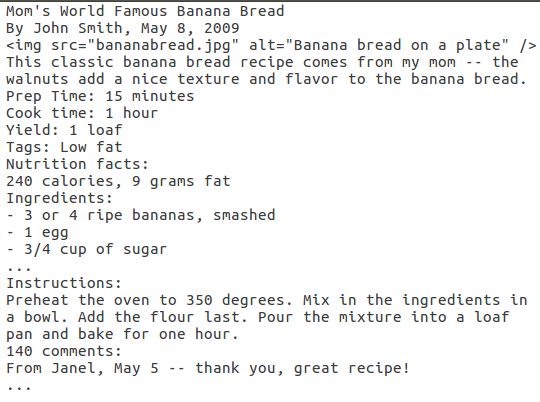
\includegraphics[width=0.7\textwidth]{Images/schemaRecipeWithoutMarkup}
		\caption{A recipe without markup}\vspace{1em}
	\end{subfigure} \\
	\begin{subfigure}{1\textwidth}
		\centering
		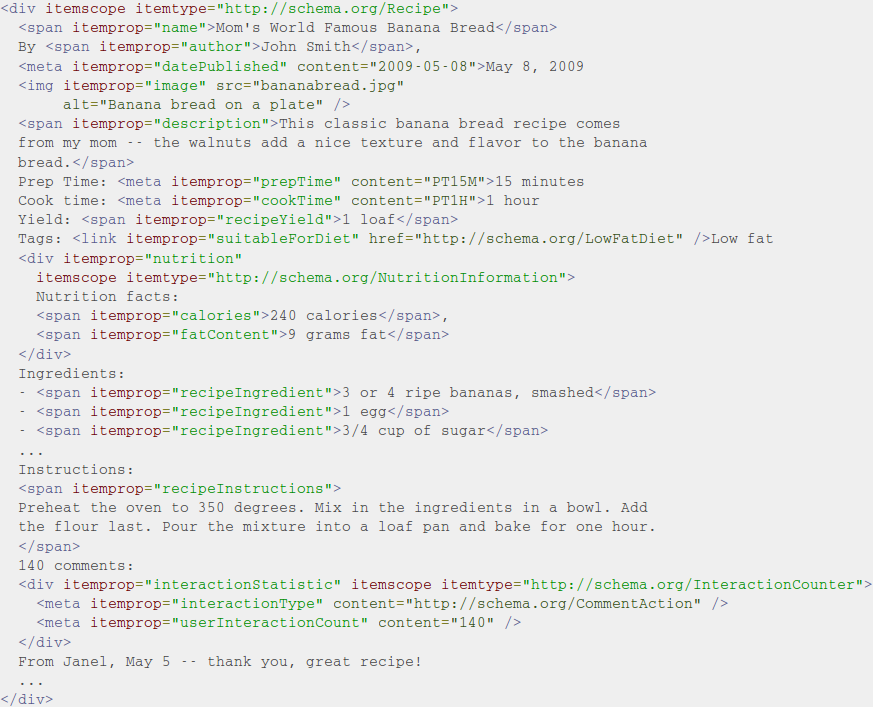
\includegraphics[width=1\textwidth]{Images/schemaRecipeWithMarkup}
		\caption{The same recipe enriched with markup}
	\end{subfigure}
	\caption{Schema.org/Recipe example from \parencite{schemaOrg}}
	\label{fig:schemaOrgRecipe}
\end{figure}


That is why we came up with \textbf{culinary editions markup language (cueML)}. It is pronounced like Kümmel, which is the German word for caraway. CueML extends TEI, retaining the goals and advantages of TEI this way. Its vocabulary sticks close to Schema.org/Recipe, so that it profits from the already established schema and can easily be transformed into it, for the sake of search engines. The main refinements are:

\begin{itemize}
	\item Add attributes for quantity and unit.
	\item Allow to mark an ingredient as optional through an additional attribute.
	\item The ability to specify that some ingredients are an alternative to each other.
	\item Distinction between basic ingredients like salt and complex ingredients like dumplings.
	\item Comprehend ingredients as unique resources, with possible different form of appearance.
\end{itemize}

The last point may seem unremarkable but enables a lot. Imagine there would be an freely available set of unique ingredient resources, which specify extra information like its nutrition information and a taxonomy categorisation like is-vegetable. Having the unique resource identifier (URI) of each ingredient from a recipe, its further processing like specifying its fat-level or if it is suitable for a diet becomes trivial, transparent and comparable to other ratings. The only thing you have to do, is collecting the freely available information of your URIs. Unfortunally we could not find such a set of resources. Therefore we used the Bundeslebensmittelschlüssel\footnote{https://www.blsdb.de/} as first approach, which we could contain with a non-public academic license. The different form of appearance is important, because for example Midder, Kalbsmidder, Kalbsmilch and Bries all describe the same ingredient in German.

A full example is shown on the next two pages. \Cref{fig:B16Scanned} is a scan of a recipe from our printed cookbook. In \cref{fig:ingredientList} is a excerpt, of how we define ingredient resources and \cref{fig:B16Enriched} shows the digital with cueML enriched version of the same recipe.

Schema.org/Recipe is not a well defined grammar. They state "some data is better than none", meaning, that they tolerate wrong meta data for reducing the risk of getting no meta data at all. Furthermore it should be easier to extend the language without an existing grammar. \parencite{schemaOrg}\footnote{at http://schema.org/docs/datamodel.html} That is obvious true, because you cannot break, what is not defined. But in contrast to them we defined cueML in a RELAX NG-grammar, which can be found in the attached cd of this thesis. We believe a grammar is a good documentation. In addition a validation against a grammar prevents simple mistakes like typing errors, which can be easily done, when tagging a lot of data.

\newpage
\begin{figure}[H]
	\centering
	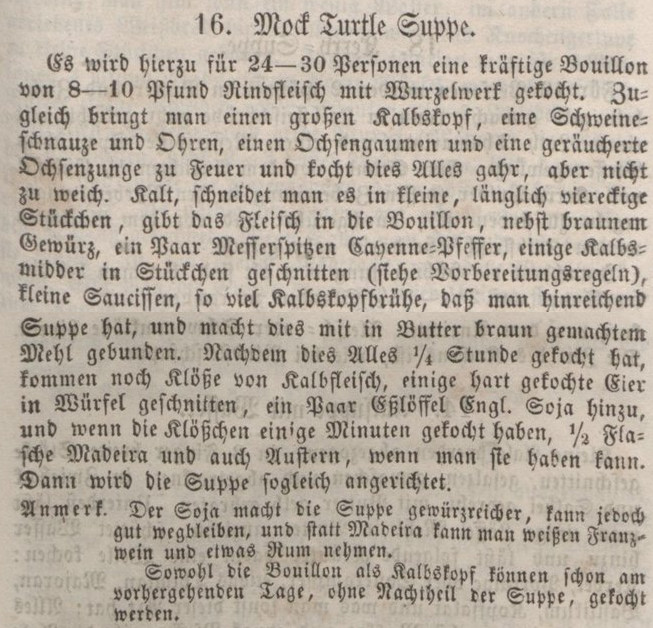
\includegraphics[width=1\textwidth]{Images/B-16}
	\caption{Recipe B-16 scanned \parencite{DTA}}
	\label{fig:B16Scanned}
\end{figure}

\begin{figure}[H]
	\centering
	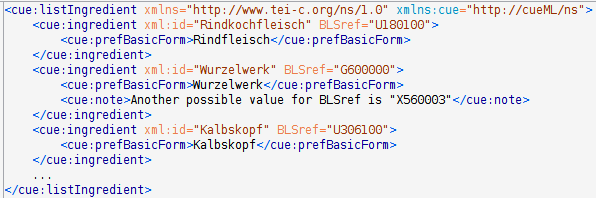
\includegraphics[width=1\textwidth]{Images/ingredientList}
	\caption{excerpt of ingredient elements}
	\label{fig:ingredientList}
\end{figure}

\newpage
\begin{figure}[H]
	\centering
	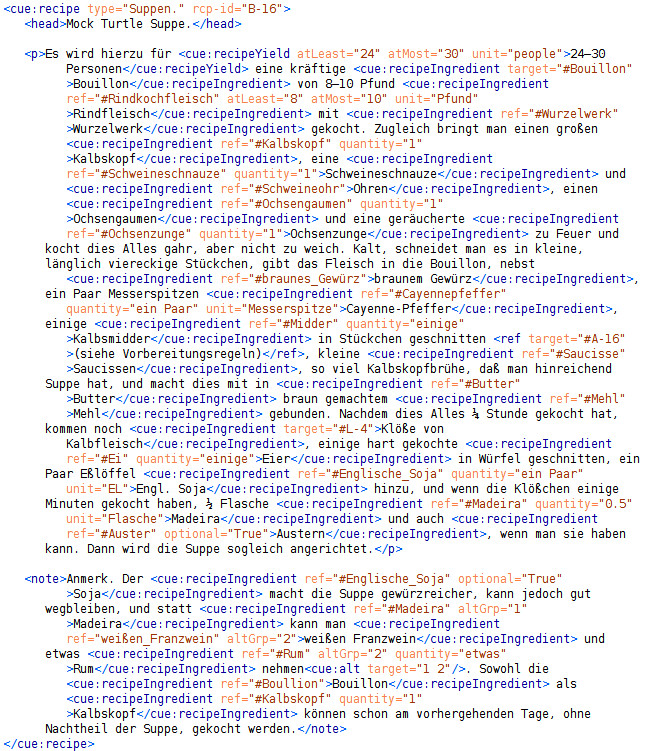
\includegraphics[width=1\textwidth]{Images/B-16-enriched}
	\caption{Recipe B-16 enriched with cueML}
	\label{fig:B16Enriched}
\end{figure}
\newpage



\section{Need for automation}\label{sec:NeedForAutomation}
The tagging requires some domain knowledge. For example we first assumed that the ingredient "Scorzoner Wurzel" is burgundy truffles. But when we realized, that it should be put into many soups, we started to doubt that. We now reason, that "Scorzonera hispanica" is meant, which is the name of salsify. Another example is bouillon. Today we would simple buy bouillon powder in the super market and mix it with water. But at the time of our cookbook it was common to cook one from the scratch and therefore there is an instruction for bouillon. Beside the cooking domain knowledge also some XML comprehension is needed for the tagging.

For tagging one recipe in our cookbook I need about 5 minutes in average. That means, that I would need more than 2 weeks of full time work, for tagging about 1000 recipes. We had a student assistant, who has never worked with XML before. In about 18 hours she could tag 66 recipes, meaning she needed more than 15 minutes in average per recipe. To be fair, her average speed would be probably better now, after she got used to XML.

Beside the needed domain knowledge and time effort, the tagging is also error prone. Looking over the tagged recipes, I found mistakes, some done by me and some more done by our student assistant.

That tagging is time consuming and error prone get emphasised by \parencite{manualTagging} as well as by the New York Times's approach to extract ingredients from recipes, which we will present in section \ref{sec:crfzeit}.

Hence automation, which has to be configured only once and can be applied to many resources afterwards, is clearly preferable.



\chapter{Related Work}
In general there exist many works about extracting useful information from textual and unstructured resources. The superordinate term for this field of research is Text Mining. It was first mentioned in \parencite{KDT} and an overview can be found in \parencite{surveyOfTextMining}. 

The algorithms for extracting useful information depend highly on existing semi-structures, which can be taken advantage of. Here we present existing algorithms, which we found in the domain of cooking, and distinct their effort from this thesis.

\section{Skip The Pizza}
\parencite{REgutGenug} is a project described on WordPress.org. The author wants to combine his two hobbies cooking and software engineering. For being able to answer questions like "How many ingredients does a typical recipe consist of?" or "Which are the most frequent ingredients?", he extracts the ingredients of recipes from the open source platform http://recipes.wikia.com/wiki/Recipes\_Wiki.

The recipes have a consistent internal representation, which is shown in \cref{lst:recipeWiki}. The semi-structure, that after \texttt{== Ingredients ==} comes a list of ingredients, can be recognized easily. Per line is one ingredient enclosed within \texttt{[[ingredient name]]}. Using this semi-structure a regular expression is already good enough for extracting the ingredients from these recipes. The quantities and units of ingredients are not of interest for this work. 

\begin{lstlisting}[frame=single, basicstyle=\footnotesize\ttfamily,caption={Shortened example recipe from \\ http://recipes.wikia.com/wiki/Recipes\_Wiki}, label=lst:recipeWiki]
* Makes 6 to 8 servings

== Ingredients ==
* 2 tbsp extra virgin [[olive oil]]
* 3 cloves [[garlic]], finely chopped
[...]

== Directions ==
Heat olive oil and garlic in large skillet over low heat until
garlic begins to sizzle.
Add tomatoes, [...]

[[Category:Cathy's Recipes]]
[[Category:Garlic Recipes]]
[...]
\end{lstlisting}


\section{Extracting Structured Data From Recipes Using Conditional Random Fields}\label{sec:crfzeit}
The New York Times provides a cooking website with recipes\footnote{\url{http://cooking.nytimes.com/}}. Their recipes are enriched with Schema.org/Recipes. For providing a recipe recommendation system based on ingredients, you have to extract the exact ingredients from a recipe, which is not enabled through this schema, as already discussed in \cref{sec:cueMLOntology}. Nevertheless they are able to extract them automatically. They use the provided structure from Schema.org/Recipe, that each ingredient phrase from the list of ingredients is marked as recipeIngredient, and Conditional Random Fields (CRF) for that. Their approach is described in \parencite{CRFZeit}. Hence we introduce here CRF first and afterwards outline their implementation.  

\subsection{Conditional Random Fields}
Given a vector of words, CRF wants to predict a suitable vector of labels. For example when the vector of words is \textit{[1 tablespoon salt]}, we want to predict \textit{[QUANTITY, UNIT, INGREDIENT]}, meaning 1 is a quantity, tablespoon a unit and salt an ingredient.

A detailed introduction to CRF can be found in \parencite{CRFIntroduction}. Here we only want to give a quick overview about linear-chain CRF, because that is the algorithm the New York Times uses. Therefore, when we write CRF, we mean linear-chain CRF.

Its starting point are vectors of words $X$, which have already correct vectors of labels $Y$. Such related sets of vectors are called training data. A joint probability distribution can be extracted from this training data, which states how likely a vector of words has a corresponding vector of labels. Taking the simplified assumption, that each label depends only on the previous label and that the current word depends only on the current label, leads to \cref{eq:jointProb}. This can always be transformed into the form of \cref{eq:magicTransoformation}. The division with $Z(X,Y)$ ensures, that the value of $p(X,Y)$ is between zero and one. $1_{condition}$ is a function, which is one if the condition is true and zero otherwise. Smart indexing leads to \cref{eq:smartIndexing}. Each $f_k$ is called a feature function. The calculation of the $\Theta_k$'s is a mathematical optimisation problem. Note that there is very likely no exact solution due to the simplified assumption of \cref{eq:jointProb}.

\begin{equation} \label{eq:jointProb}
p(X,Y) = \prod_{t=1}^T p(y_t|y_{t-1}) * p(x_t|y_t), \quad T = \#X
\end{equation}
\begin{align}\label{eq:magicTransoformation}
p(X,Y) = \frac{1}{Z(X,Y)}\prod_{t=1}^T exp(\sum_{i,j\in S}^{} \Theta_{i,j} * 1_{y_t=i} * 1_{y_{t-1}=j} + \sum_{i \in S}^{} \sum_{j \in O}^{} \mu_{o,i} * 1_{y=i} * 1_{x_t=o}), \nonumber
\\
Z(X,Y) = \sum_{X}^{}\sum_{Y}^{}\prod_{t=1}^T exp(\sum_{i,j\in S}^{} \Theta_{i,j} * 1_{y_t=i} * 1_{y_{t-1}=j} + \sum_{i \in S}^{} \sum_{j \in O}^{} \mu_{o,i} * 1_{y=i} * 1_{x_t=o}), \nonumber
\\
S = all\ possible\ labels, \quad O = all\ possible\ words
\end{align}
\begin{align} \label{eq:smartIndexing}
p(X,Y) = \frac{1}{Z(X,Y)}\prod_{t=1}^T exp(\sum_{k=1}^{K} \Theta_{k} * f_k(y_t, y_{t-1}, x_t)), \nonumber
\\
Z(X,Y) = \sum_{X,Y}^{}\prod_{t=1}^T exp(\sum_{k=1}^{K} \Theta_{k} * f_k(y_t, y_{t-1}, x_t))
\end{align}

A joint probability distribution can always be transformed into a conditional probability as shown in \cref{eq:condProb}.

\begin{equation}\label{eq:condProb}
p(Y|X) = \frac{p(X,Y)}{\sum_{Y'\in S}^{}p(Y', X)}
\end{equation}

The described model so far is a Hidden Markov Model. In a CRF you are also allowed to take only a subset of these features, what can improve performance without loosing accuracy. Additional improvement in a CRF can very likely be achieved by further custom feature functions, which may depend on the whole vector of words, instead of only the current word identity. For example some custom feature functions could be:

\begin{itemize}
\item $f_{k+1}(y_t, y_{t-1}, X) = 1_{x_t\ starts with\ upper\ case}$
\item $f_{k+2}(y_t, y_{t-1}, X) = 1_{x_t\ is\ in\ a\ domain\ specific\ dictionary}$
\item $f_{k+3}(y_t, y_{t-1}, X) = 1_{x_t\ is\ in\ a\ domain\ specific\ dictionary\ and\ x_{t-1}\ is\ an\ article}$
\end{itemize}

Putting all together leads to \cref{def:defCRF}. Note that after plugging \cref{eq:smartIndexing} into \cref{eq:condProb} $Z$ now only depends on $X$.

\begin{defn}[linear-chain Conditional Random Field] \label{def:defCRF}
    A linear-chain Conditional Random Field is a conditional distribution of the form: \vspace*{0.5em} \\
    $p(Y|X) = \frac{1}{Z(X)}\prod_{t=1}^T exp(\sum_{k=1}^{K} \Theta_{k} * f_k(y_t, y_{t-1}, X))$, where \\
    \hspace*{2em}$Z(X) = \sum_{S}^{}\prod_{t=1}^T exp(\sum_{k=1}^{K} \Theta_{k} * f_k(y_t, y_{t-1}, X))$ and \\
    \hspace*{2em}$Y$ vector of labels, $X$ vector of words, $S$ set of all possible labels
\end{defn}

Having a CRF in place, a natural prediction function is shown in \cref{eq:CRF}. The calculation of $prediction(X)$ can be done in $(\#S)^2*\#X$ through dynamic programming techniques.

\begin{equation}\label{eq:CRF}
prediction(X) = argmax_Y(P(Y|X))
\end{equation}

\subsection{Implementation of New York Times}
As starting point the New York Times have manually specified labels for over 130,000 ingredient phrases, which they use as training data. They are extracted out of their website, where their recipes are already enriched with Schema.org/Recipe.

One example ingredient phrase is shown in \cref{lst:NYTTrainingData}. They use CRF++\footnote{\url{https://taku910.github.io/crfpp/}} as library, which is an implementation of CRF. The first word per column is the actual word. The last word is the label, which should be predicted in IOB2 format. The format states, that the beginning of an entity gets prefixed with \textit{B-} and the continuation with \textit{I-}, as you can see in the last three words. Words, which do not belong to a relevant entity, get labelled with \textit{OTHER}. The labels in between are custom features. 

\begin{lstlisting}[frame=single, caption={Extract of the training data for New York Times CRF}, label=lst:NYTTrainingData]
3/4       I1  L12	 NoCAP	NoPAREN	 B-QTY
pound     I2  L12	 NoCAP	NoPAREN	 OTHER
shiitake  I3  L12	 NoCAP	NoPAREN	 B-NAME
mushrooms I4  L12	 NoCAP	NoPAREN	 I-NAME
,         I5  L12	 NoCAP	NoPAREN	 OTHER
stemmed   I6  L12	 NoCAP	NoPAREN	 B-COMMENT
and       I7  L12	 NoCAP	NoPAREN	 I-COMMENT
quartered I8  L12	 NoCAP	NoPAREN	 I-COMMENT
\end{lstlisting}

The feature functions, which the CRF should use, are specified through the templates of \cref{lst:NYTfeatureTemplates}. They have the format \textit{U00:\%x[row,column]}. The row specifies the targeted word in relative position to itself and the column specifies the absolute position. Therefore when the actual word is mushrooms the data from \cref{lst:NYTTrainingData} would be expended to the values in \cref{lst:NYTfeatureTemplatesDerivedValue}.

\newpage
\begin{minipage}{0.4\textwidth} 
\begin{lstlisting}[frame=single, caption={Feature templates for New York Times CRF}, label=lst:NYTfeatureTemplates]
# Unigram               
U00:%x[-2,0]             
U01:%x[-1,0]              
U02:%x[0,0]
U03:%x[1,0]
U04:%x[2,0]
U05:%x[0,1]
U06:%x[0,2]
U07:%x[0,3]

U08:%x[-2,4]
U09:%x[-1,4]
U10:%x[0,4]
U11:%x[1,4]
U12:%x[2,4]

U13:%x[0,0]/%x[0,2]
U14:%x[0,1]/%x[0,2]
U15:%x[0,0]/%x[0,3]
U16:%x[0,0]/%x[0,4]
U17:%x[0,0]/%x[0,1]

# Bigram
B
\end{lstlisting}
\end{minipage}
\hfill
\begin{minipage}{0.5\textwidth} 
\begin{lstlisting}[frame=single, caption={Derived values when the current word in \cref{lst:NYTTrainingData} is mushrooms}, label=lst:NYTfeatureTemplatesDerivedValue]
            
pound            
shiitake            
mushrooms
,
stemmed
I4
L12
NoCAP

NoPAREN
NoPAREN
NoPAREN
NoPAREN
NoPAREN

mushrooms/L12
I4/L12
mushrooms/NoCAP
mushrooms/NoPAREN
mushrooms/I4


I-NAME B-Name
\end{lstlisting}
\end{minipage}

Feature functions are extracted from these templates and the corresponding values of the training data as shown in \cref{lst:featureFunctionExtraction}. The B-template takes the transition from $y_{t-1}$ to $y_t$ into account. Note that for example the custom feature function, if a word is inside parentheses, gets implemented through adding a label YesPAREN/NoPAREN to the trainings data in the fourth column and specifying the feature template U10\%[0,4]. Also note, that for each such template $\#(all\ possible\ labels)*\#(all\ possible\ words)$ different feature functions gets created. For the B-template $\#(all\ possible\ labels)^2*\#(all\ possible\ words)$ different feature functions gets created.

\begin{lstlisting}[frame=single, caption={Extracting of feature functions from templates}, label=lst:featureFunctionExtraction, mathescape]
U02:%[0,0]          $\rightarrow 1_{y_t=I-Name\ and\ x_t=mushrooms} $
U02:%[-2,4]         $\rightarrow 1_{y_t=I-Name\ and\ x_{t-2}\ 4th\ label\ is NoPAREN} $
U13:%x[0,0]/%x[0,2] $\rightarrow 1_{y_t=I-Name\ and\ x_t=mushrooms\ and\ x_t\ 2nd\ label\ is L12} $

B                   $\rightarrow 1_{y_t=A\ and\ y_{t-1}=B}\ for\ each\ A,B\ \in\ possible$
                                               $prediction\ labels$
\end{lstlisting}

Hence the only custom features the New York Times take into account for prediction are the word identity (column 0), the index of the current word (column 1), the length of the sentence (column 2, rounded to 4, 8, 12, 16 or 20), if the word starts capitalized (column 3) and if the word is inside parenthesis (column 4), in relation with the current word and some surrounding words.

When applying their algorithm to 481 example recipes, they get 89\% sentence-level accuracy, meaning that they get 9 out of 10 ingredient phrases completely right. They tested only so few recipes, although they had over 130,000 ready labeled recipes, because they found no way for automatic evaluation. Their problem was, that there were to many ambiguous phrases and to many mistakes in the manually labeled data.
 
 
\section{Domain Specific Information Extraction for Semantic Annotation}
\parencite{GrammaBased} is a diploma thesis about extracting ingredients and their further processing from recipes. Their algorithm could be divided into two main parts.

First to check every word, if it is in a dictionary of ingredients respectively a dictionary of actions and label it accordingly. For keeping the dictionaries as small as possible they do a morphological Analysis and only store the lemmas of the words. The second main part, and more sophisticated task, is to identify, which action should be applied to which ingredient. They have a rule based approach and a dependency parsing based approach for that.

The rule based approach is to do a part of speech tagging (POS) first and afterwards try to apply a small set of rules, which define a context free grammar, with predefined meaning. \Cref{lst:ruleBased} shows an example, meaning buttermilk and bananas should be added.

\begin{lstlisting}[frame=single, basicstyle=\footnotesize\ttfamily,caption={Rule based example}, label=lst:ruleBased, mathescape]
# Example sentence
add buttermilk and bananas

# Example sentence with POS and dictionary-label
add[ACT] buttermilk[ING] and[CC] bananas[ING]

# Apply rule VP -> ACT NP (,NP)* (CC NP)?
# Predefined meaning of the rule: Apply ACT to all ING  
-> ACT NP CC NP
# Apply rule NP -> DT? JJ* ING twice  
-> ACT ING CC ING

# With: 
# VP,NP $\in$ non-terminal symbols, CC $\in$ Conjunctions, DT $\in$ Determiner, ACT := action, ING := ingredient
\end{lstlisting}

The second approach is to do a dependency based parsing, which represents the semantic structure of a sentence in a tree like format. For example \cref{fig:johnLikesApple} represents, that the subject of like is John and the liked object is Apple.
The format as well as building the tree is way more complex than the previous simple rules, but the tree can be build by already existing tools like the Stanford Parser\footnote{\url{http://nlp.stanford.edu/software/lex-parser.shtml}}. The semantic structure of the sentences give strong evidence, which action should be applied to which ingredient.

\begin{figure}[H]
	\centering
	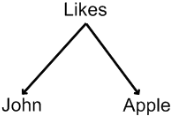
\includegraphics[]{Images/JohnLikesApple}
	\caption{John likes apple \parencite{GrammaBased}}
	\label{fig:johnLikesApple}
\end{figure}

In their evaluation they apply these two variants to 43 randomly selected recipes from the internet. Their precision and recall are presented in table \ref{tab:masterEval}. Even the more sophisticated dependency based approach has only a recall of 64\%. This is due to a lack of mapping actions to their corresponding ingredients.

\begin{table}[H]
	\centering
	\begin{tabular}{ l | c | r } 
		& Precision & Recall \\
		\hline
		Rule based & 97.39\% & 51.54\% \\
		Dependency Based & 95.4\% & 64.12\% \\
	\end{tabular}
	\caption{Evaluation Domain Specific Information Extraction for Semantic Annotation}
	\label{tab:masterEval}
\end{table}


\section{Data-driven Knowledge Extraction for the Food Domain}
\parencite{konvens07_wiegand12o} are interested in relations of ingredients. They analyse the four relations:
\begin{enumerate}
	\item INGREDIENT typically suits to EVENT
	\item INGREDIENT is typically served with other INGREDIENT
	\item INGREDIENT can be replaced with other INGREDIENT
	\item INGREDIENT is part of RECIPE
\end{enumerate}

Their data set consists of pure text, divided into title and body. They use GermaNet\footnote{\url{http://www.sfs.uni-tuebingen.de/GermaNet/}} for the extraction of ingredients. GermaNet is a thesaurus for German words providing a category "Nahrung", which means food. When the lemma of a word appears in this category, the word is assumed to be an ingredient. They have three for us relevant methods for instantiating their relations. We only cover their  connection the relation \textit{Ingredient is part of recipe}, because that is the one we are interested in.

\textbf{Title and body} instantiates for each ingredient of a body a relation, if the title is a recipe. This way they reach a P@10 of 0.776, meaning that when ask for the ingredients of a recipe almost 8 of 10 are right. We want to mention, that this value is a lower boundary. For example when a recipe consists only of 5 ingredients, the maximal possible P@10 value would be 0.5.

The other two methods are \textbf{Pattern-based} and \textbf{Co-occurrence}. Both evaluation are very bad and therefore we only discuss the idea of them. Pattern-based searches for patterns like \textit{RECIPE made of INGREDIENT}. They state, that when a pattern is matched, it is always a good match, but that they match not often. They also state, that patterns, based on dependency based parsing, like in the previous section, are not an improvement, due to domain specific mismatch of the parser. Co-occurrence looks for co-occurrences in the text of a recipe and an ingredient.

Last they note, that the relations 2 and 3 are often mixed-up, because they are very similar to each other.
 


\section{Lessons for this work}
\parencite{REgutGenug} exploits a strict semi-structure, which is not given in our very unstructured cookbook. Therefore we need more advanced algorithm than regular expressions.

\parencite{CRFZeit} take advantage of the point, that they have already marked the ingredient phrases from the list of ingredients. But our cookbook has no list of ingredients. Nevertheless, the ingredient phrases could be extracted from plain text through a CRF algorithm first and afterwards we could use the algorithm of \parencite{CRFZeit}. Another option would be to just try a CRF on the plain text guessing all the work at once. However we have to consider, that we do not have near as 130,000 training data. Our lack of training data could be caught up by more sophisticated custom feature functions.

\parencite{GrammaBased} only uses plain text. But they have a bad recall, due to the point, that they are not good in mapping actions to their corresponding ingredients. In contrast to mapping actions to ingredients, we want to map quantities to units and these in turn to ingredients, which could be an easier task. Anyway, the dictionary check, enabled by a morphological analysis, from their algorithm first main part, could be a good  custom feature function for a CRF.

\parencite{konvens07_wiegand12o} is interesting, because we target recipes and therefore can easily do their Title and body method. They also enforce \parencite{GrammaBased}, that pattern-based extraction is good, when the patterns match, what is unfortunately not often the case. The Co-occurrence method is an interesting idea for categorization, if an ingredient is optional, or an alternative to another one. For example the co-occurrence of \textit{two ingredients} and the word \textit{instead} within one sentence indicate, that the two ingredients are an alternative to each other.



\chapter{CRF-based Extraction}
We present a very basic prototype for extracting ingredients from recipes based on CRF in this chapter.

\section{CRF prototype}
This prototype can be found under the following git tag\footnote{\url{https://github.com/Torsten89/SourceCodeExtractingRecipeIngredientsFromCookbooks/tree/FirstCRFPrototype}}. It uses the SWIG API of crfsuite\footnote{\url{http://www.chokkan.org/software/crfsuite/}} as python binding. For labeling we take the tags \texttt{B-Quantity}, \texttt{I-Quantity}, \texttt{B-Unit}, \texttt{B-Ingredient}, \texttt{I-Ingredient}, \texttt{B-CookTime}, \texttt{I-CookTime},
\texttt{B-Yield}, \texttt{I-Yield}, \texttt{B-IngredientYield}, \texttt{I-IngredientYield}
\texttt{B-Link}, \texttt{I-Link} and \texttt{O} for others. We tag 9 of our recipes with these tags. For illustrating the beginning of such a tagged recipe is shown in \cref{lst:trainingsData}. Our used features are word identity and label transitions.

\begin{lstlisting}[caption={Trainings data}, label=lst:trainingsData]
#B-1
Klare            O
weiße            O
Rindfleischsuppe O

Man	             O
rechnet	         O
,                O
wenn             O
die	             O
Gesellschaft     O
klein            O
ist              O
,                O
auf              O
jede             O
Person           O
3/4	             B-Quantity
Pfund            B-Unit
,                O
bei              O
einer            O
großen           O
Gesellschaft     O
1/2	             B-Quantity
Pfund            B-Unit
Fleisch          B-Ingredient
.                O

...
\end{lstlisting}


\section{Evaluation of this prototype}
Although this is only a simple prototype, it raises many questions.

First we do a little test on a recipe from our cookbook, which was not in the training data. It can be found in \cref{appendix:crfTraini}. It consists of 96 words. From these 96 words the CRF got all 83 \texttt{O}-tags correctly. From the 13 tags other than \texttt{O} it missed the 5 shown in \cref{lst:crfResult}. \textit{Eine} and \textit{einige} means \textit{some} and is a vague quantity. The other three are potatoes and potato dumplings.

\begin{lstlisting}[caption={Differences}, label=lst:crfResult]
eine            B-Quantity      O
einige          B-Quantity      O
Kartoffeln      B-Ingredient    O
Kartoffeln      B-Ingredient    O 
Kartoffel-Klöße B-Ingredient    O
\end{lstlisting}

\textit{Eine} and \textit{einige} appear very often in German and are only sometimes the quantity of an ingredient. Therefore it is hard for a CRF to get this right. But because the quantity is vague, it is questionable to mark it anyway.

Potatoes could be likely caught through a custom feature function $1_ {word\ is\ in\ dictionary\ of\ ingredients}$. But having that in place, one has to ask for the advantage of the CRF, when we can already extract the ingredients with a dictionary.

We decided to not follow up the CRF approach, because we bothered with following limitations, as we reasoned about the CRF:

\begin{itemize}
	\item Further feature and label engineering is not straight forward. First of all we have only considered ingredients. For optional ingredients as well as for alternative ingredients two new labels are required. Also sometimes a recipe introductions tells you to not use an ingredient, which could be marked with an own label. But these four
	labels are very similar, and therefore the CRF probably needs more features to distinguish between them. One such a feature could be, if \textit{don't} is within the sentence.
	(Time consuming!)
	\item A CRF is not able to extract relations between entities. Once the ingredients, quantities and units are extracted, they still have to be matched together. Also when ingredients are marked as alternative ingredients, it is still unclear which one are an alternative to which.
	\item Only labeling ingredients is a simplification of our cueML. We would also like to distinguish between basic and complex ingredients. When it is a basic ingredient, we would like to add a reference to the Bundeslebensmittelschlüssel. And when it is a complex ingredient, we would like to add a reference to a recipe of it. Also breaking down, what kind of meat, when a sentence only mentions meat, is not possiblle within the CRF.
	\item Above all a further development is to time consuming for this master thesis. The 9 trainings recipes lead to more than 1400 lines, which have to be tagged manually. Assuming 10 seconds per line, that would take more than three hours. 10 seconds may seem pessimistic, but consider the following translated example from our cookbook: \textit{Take the veal as in number one, according to the number of people take a little bit more, because it has less taste than beef.} When not reading carefully, it is easy to tag \textit{beef} as an ingredient. Building up 130,000 trainings recipes, like the NYT did, or !!!CoNLL task!!!, is not reasonable within this project.
\end{itemize}


\chapter{Dictionary- and Rule-based extraction}
First we introduce here a basic prototype, which is based upon dictionary extraction and further rule-based processing. After that we continue to develop of this approach, because we find it promising.

\section{Dictionary- and Rule-based prototype}
-lemmas mit -wurzel aufpimpung

\begin{figure}
	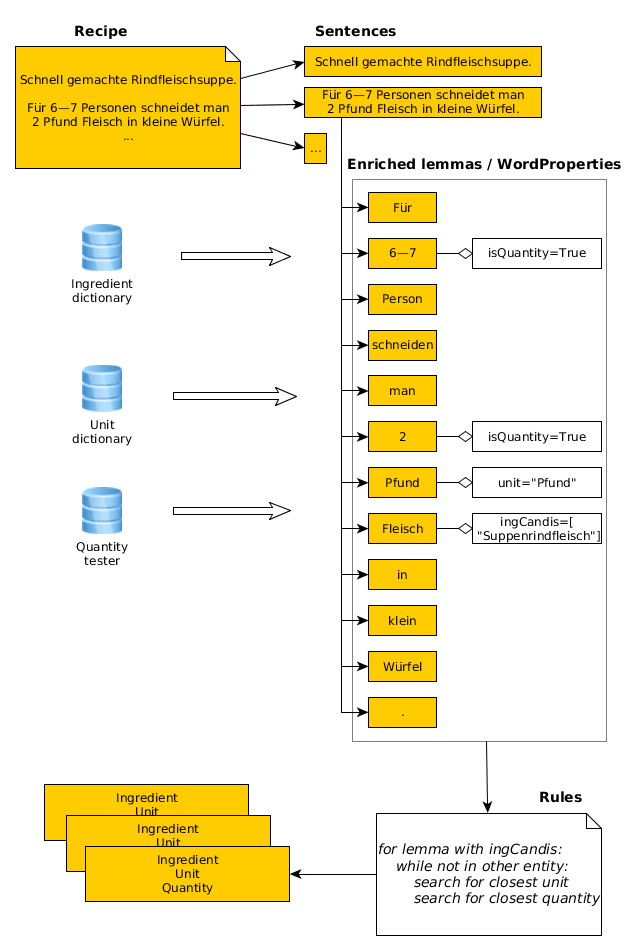
\includegraphics[width=1\linewidth]{Images/dictBasedExtraction}
	\caption{Dictionary- and Rule-based workflow}
	\label{fig:workflowDictbased}
\end{figure}


\subsection{Evaluation}
- besser testbar (testcase vs crf neue features -> funktioniert alles noch, anderes funktioniert vll besser)


\section{Evaluation}
Precision and recall are metrics, which measure the quality of an information extracting algorithm.

\begin{equation} \label{eq:precisionAndRecall}
Precision = \frac{\#(retrieved \cap relevant)}{\#retrieved}, \hspace{1em} Recall = \frac{\#(retrieved \cap relevant)}{\#relevant}
\end{equation}

They are defined as shown in \cref{eq:precisionAndRecall} according to \parencite{surveyOfTextMining}. A high precision states, that the algorithm does only find relevant information as intended. The ideal precision of one would mean, that all extracted data where useful. A high recall states, that the algorithm finds many of the total relevant information. The perfect score of one would mean, that all relevant information were found. Both are needed for the evaluation of an algorithm. If only considering precision, the algorithm could only find the information, which are obvious relevant and therefore find only view information, but having a high score this way. On the other side, if only considering recall, the algorithm could return everything. This way its score would have the perfect value of one. But both algorithm are obvious not good, which gets covered by a low value of the other formula.




%Discussion------------------------------------------------------------------%
\chapter{Discussion}

\section{Usefulness of automatic extraction of ingredients}\label{sec:UsefulnessOfThesis}
I personally feel it is an interesting computer science challenge to extract ingredients from plain text and make them machine readable. But that would be a bad justification for a master thesis. This section points out some of many applications, which are possible, once the ingredients are extracted. Building a database manual for all these applications is way to time consuming, as pointed out in \ref{sec:NeedForAutomation}. Therefore this thesis is useful, what is a good motivation as well as a good justification for this master thesis.

\parencite{recipeRecommendation} build a \textbf{recipe recommendation system} for a cooking website, based on which ingredients are liked by the users and which not.

Beside that, there seems to exist a lot of effort about \textbf{diet, targeting the well being}. \parencite{ingredientNetworks} analyse, how far a recipe is liked in relation with its nutrition information, which are based on the ingredient of the recipe. They also analyse how far an ingredient can be replaced through another ingredient, which is nice, if you want a low-fat alternative, or it is not available right now. \parencite{Freyne2010} as well as \parencite{Geleijnse_extractingvegetable} build a recipe recommendation, which prefer healthy recommendations. As before, the healthiness of a recipe is determined through its used ingredients.

Both, a recommendation system as well as help with healthy diet, do obviously increase the attractiveness of a cooking website. That raises the question, how much are these features worth. Unfortunally it is not an easy task to determine the value of cooking websites. Chefkoch.de, which is the biggest German cooking website, is a 100\% subsidiary of Gruner+Jahr today, but there are no reliable information about the cost of acquisition. They are also not allowed to share any information about their revenue, but have more than 100 employees, what is an indication for a lot of revenue (see \cref{appendix:emailChefkoch}). Therefore these application are probably also worth a lot.


\textbf{Social science} is also possible through analysing recipes. For example \parencite{BeateHenning} analyses typical characteristics of cookbook through German history. She noticed that recipes before the 18.th century often contained ingredients, which should mask the taste of rotted food, what is clearly a sign for poverty and food shortage. Fasting meals covered about a third of many cookbooks, which emphasises the influence of the church at that time. First mentions of non-native ingredients and meals are indications for intercultural exchange. Rare and expensive ingredients are signs for prosperity while possible substitution of them for poverty. Another example is in \parencite{FlavorNetwork}. They compare American and Asian culinary practice based on about 56.000 recipes.


\section{Contribution to field of research}
- rule-based nicht exakt match sondern co-occurrence von Indikationswörtern (Ingredients und "anstatt")
- Übertragung auf beliebige / allgemeine Rezepte


\section{Quality of cueML and the obtained data}
- Mengenangaben ohne recipeYield witzlos
- Übersetzung von (historischen) Mengenangaben (Maß)
- ganzes Gewürz
- Ungenaue Mengenangaben (ein Stich, 5Pfennig Brot, etwas)
- links/refs erschweren Auswertung
- BLS Angaben für alk. freie Getränke :D :D :D, nicht open source, nicht word wide
- welche Zutat welche BLS key (BLS überraschend schwer :D)
-In B-2 "Anmerk. Will man Reis oder Sago zur Suppe nehmen, so gibt man dieses später
hinein. Man rechnet davon auf jede Person bei allen Fleischsuppen einen gestrichenen Eßlöffel voll."

Infos aus Allg. Vorteil eines Kapitels (Reis 15g pro Suppe)

-Mensch kann Fehler erkennen (B-10 Rindfleisch ->Hasen /falscher Vreweis)

- Publishen / Sharen von cueML
	- \parencite{GrammaBased} also points out that ontology building is time consuming and expensive
	- Schema alignment paper - nicht ein schema für alle Zwecke

\section{Rapid Prototyping}
- TDD / früh Plausibilitäts-Überprüfungen - Tagen als Hi-Wi war ne dumme Aktion^^ (insbesondere fürs Schemata, Mengenangaben und Namen historische Recherche nötig (Gefühl für die Daten, Wurzelwerk, braunes Gewürz,	Engl. Soja, tagging schema ist schwieriger als gedacht))
- CRF zu aufwändig 

\section{Knowledge is power}
The goal of the following digression is to provide some critical though and to sensitize for the importance of data privacy. Due to the point that the goal of this overall thesis is to facilitate some machine readable data, and machine readable data provides a lot of knowledge per definition of itself, this is an important personal concern of me. Because this is not a thesis in humanities, I feel free to over exaggerate a little bit and use sources like Wikipedia here.

According to Wikipedia \footnote{\url{https://en.wikipedia.org/wiki/Scientia_potentia_est} visted on 01/10/17} the first recorded occurrence of the proverb "Knowledge is power" is already from the tenth-century stating \textit{"Knowledge is power and it can command obedience. A man of knowledge during his lifetime can make people obey and follow him and he is praised and venerated after his death. Remember that knowledge is a ruler and wealth is its subject"}. How this thesis can support wealth was already discussed in \cref{sec:UsefulnessOfThesis}.

But \textbf{with great power comes great responsibility}\footnote{A well known proverb which probably has its origin from the French National Convention during the period of French Revolution. (\url{http://quoteinvestigator.com/2015/07/23/great-power/} visited on 11/02/16)}. I want to give two examples, where knowledge provided through data had/have terrifying power:

First, the Weimar Republic changed 1919 their constitution, giving the state the right to acquire the religion affiliation of their citizen in a census. That makes sense, because the state does collect the church taxes for the catholic church in Germany and therefore has to know, who is catholic. 1939 the regime of Adolf Hitler used that right, to enforce everybody to tell if they self, one of their parents or one of there grandparents are Jews, leading to a categorization of full Jew, hybrid of level one or hybrid of level two. It is uncertain today, how far the regime used these data, to deport people into concentration camps\footnote{\url{https://de.wikipedia.org/wiki/Volkszählung_im_Deutschen_Reich_1939} visted on 28/12/16}. But in my opinion it is easy to imagine, that they did take use of these information in some way. Otherwise they would not have collected it. And even the possibility that the religion of one of your grandparents could lead to deportation into a concentration camp, frightens me, that insane regimes could do anything with any data.

Second it is actual very present in the media, how far "faked news" influence elections\footnote{e.g \url{https://www.nytimes.com/2016/11/18/technology/fake-news-on-facebook-in-foreign-elections-thats-not-new.html?_r=0} visted on 12/11/16}, adjudging news, which are some sort of data and knowldege, huge power. Also very present is the claim, that Russia has collected material to blackmail the next American president Donald Trump\footnote{\url{https://www.nytimes.com/2017/01/10/us/politics/donald-trump-russia-intelligence.html} visted on 10/01/17}. This ability is also clearly very powerful. I personally would be surprised, if they had not done that, because the western countries do the same to some point. The Global surveillance disclosures revealed that the American and British secret services monitored huge parts of the internet\footnote{\url{https://en.wikipedia.org/wiki/Global_surveillance_disclosures_(2013-present)} visited on 11/01/17}. I am convinced, that this is very expensive and that one payback is the hope to find material, they can use for their political advantage. For example the mobile phone of the German chancellor was monitored since 2002\footnote{\url{http://www.spiegel.de/politik/deutschland/handy-der-kanzlerin-die-wichtigsten-fakten-der-abhoeraffaere-a-930411.html} visited on 11/01/17}. It takes not much imagination to associated that with the declining of the Iraq War of the actual chancellor as well as with his closeness to Russia at that time.

In the context of a program, which make recipes machine readable, this all might be total exaggerated. But the health of Hillary Clinton was a topic at the American president election 2016\footnote{\url{https://www.washingtonpost.com/news/the-fix/wp/2016/09/11/hillary-clintons-health-just-became-a-real-issue-in-the-presidential-campaign/} visted on 02/11/16}. I personal know, that you should not eat some ingredients, when you have pancreatic cancer, which gets underlined by forum questions\footnote{\url{http://www.chefkoch.de/forum/2,51,639082/Bauchspeicheldruesen-rezepte.html} visited on 11/02/17}. It probably would have had effected survey results, when someone, who favoured Donald Trump, had tracked Hillary's internet traffic and stated Hillary had pancreatic cancer, based on the fact, that she was interested in recipes, avoiding these ingredients. I also wonder, if revealing Hillary were a vegetarian would have had a bad impact on her survey results. 

As mentioned at the top, this section was not very scientific. But I hope, that I could provide some critical thoughts, keeping in mind.


\chapter{Summary}


\appendix
\chapter{Statutory Declaration}
I declare that I have developed and written the enclosed Master Thesis completely by myself, and have not used sources or means without declaration in the text. Any thoughts from others or literal quotations are clearly marked. The Master Thesis was not used in the same or in a similar version to achieve an academic grading or is being published elsewhere.
\newline
\newline
\newline
\rule{\textwidth}{1pt}
Location, Date \hfill Signature 

\chapter{Emails with Chefkoch.de} \label{appendix:emailChefkoch}
\vspace{-1cm}
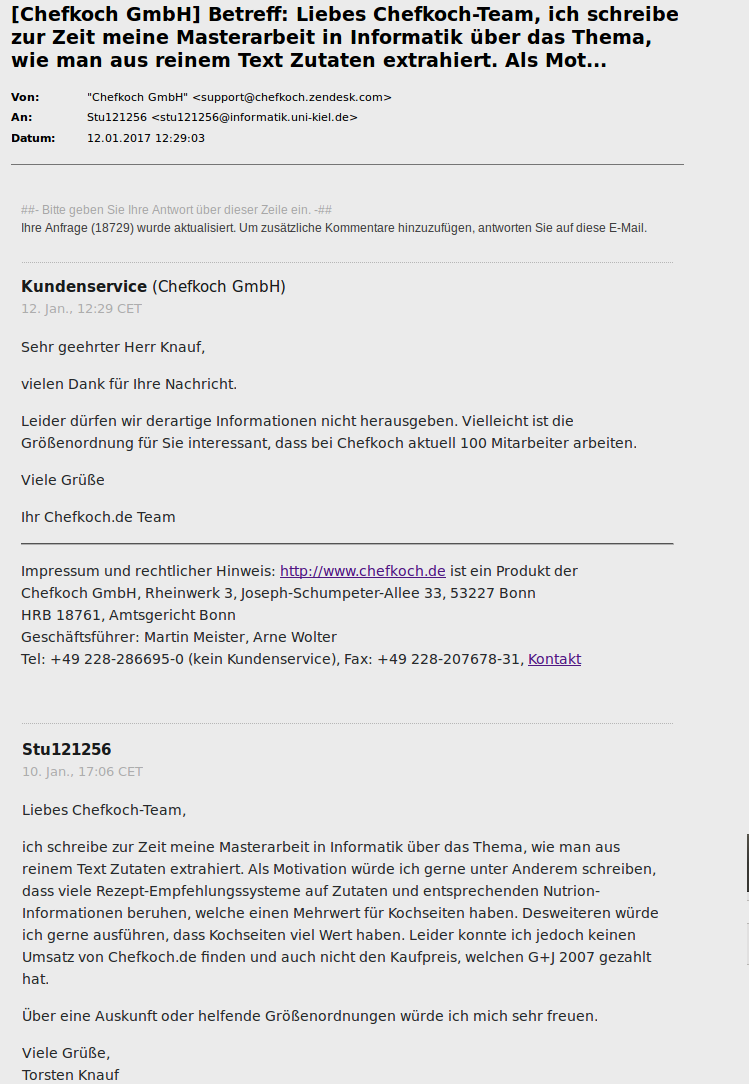
\includegraphics[width=1\linewidth]{Images/emailChefkoch}

\printbibliography

\chapter{For CRF tagged trainings recipe} \label{appendix:crfTraini}
\begin{lstlisting}
#B-16                
Mock                O
Turtle              O
Suppe               O

Es                  O
wird                O
hierzu              O
für                 O
24                  B-Yield
-                   I-Yield
30                  I-Yield
Personen            O
eine                O
kräftige            O
Bouillon            B-Ingredient
von                 O
8                   B-Quantity
-                   I-Quantity
10                  I-Quantity
Pfund               B-Unit
Rindfleisch         B-Ingredient
mit                 O
Wurzelwerk          B-Ingredient
gekocht             O
.                   O

Zugleich            O
bringt              O
man                 O
einen               B-Quantity
großen              O
Kalbskopf           B-Ingredient
,                   O
eine                B-Quantity
Schweineschnauze    B-Ingredient
und                 O
Ohren               B-Ingredient
,                   O
einen               B-Quantity
Ochsengaumen        B-Ingredient
und                 O
eine                B-Quantity
geräucherte         O
Ochsenzunge         B-Ingredient
zu                  O
Feuer               O
und                 O
kocht               O
dies                O
Alles               O
gahr                O
,                   O
aber                O
nicht               O
zu                  O
weich               O
.                   O

Kalt                O
,                   O
schneidet           O
man                 O
es                  O
in                  O
kleine              O
,                   O
länglich            O
viereckige          O
Stückchen           O
,                   O
gibt                O
das                 O
Fleisch             B-Ingredient
in                  O
die                 O
Bouillon            B-Ingredient
,                   O
nebst               O
braunem             B-Ingredient
Gewürz              I-Ingredient
,                   O
ein                 B-Quantity
Paar                I-Quantity
Messerspitzen       B-Unit
Cayenne-Pfeffer     B-Ingredient
,                   O
einige              B-Quantity
Kalbsmidder         B-Ingredient
in                  O
Stückchen           O
geschnitten         O
(                   B-Link
siehe               I-Link
Vorbereitungsregeln I-Link
)                   I-Link
,                   O
kleine              O
Saucissen           B-Ingredient
,                   O
so                  O
viel                O
Kalbskopfbrühe      O
,                   O
daß                 O
man                 O
hinreichend         O
Suppe               O
hat                 O
,                   O
und                 O
macht               O
dies                O
mit                 O
in                  O
Butter              B-Ingredient
braun               O
gemachtem           O
Mehl                B-Ingredient
gebunden            O
.                   O

Nachdem             O
dies                O
Alles               O
1/4                 O
Stunde              O
gekocht             O
hat                 O
,                   O
kommen              O
noch                O
Klöße               B-Ingredient
von                 I-Ingredient
Kalbfleisch         I-Ingredient
,                   O
einige              B-Quantity
hart                O
gekochte            O
Eier                B-Ingredient
in                  O
Würfel              O
geschnitten         O
,                   O
ein                 B-Quantity
Paar                I-Quantity
Eßlöffel            B-Unit
Engl.               B-Ingredient
Soja                I-Ingredient
hinzu               O
,                   O
und                 O
wenn                O
die                 O
Klößchen            B-Ingredient
einige              O
Minuten             O
gekocht             O
haben               O
,                   O
1/2                 B-Quantity
Flasche             B-Unit
Madeira             B-Ingredient
und                 O
auch                O
Austern             B-Ingredient
,                   O
wenn                O
man                 O
sie                 O
haben               O
kann                O
.                   O

Dann                O
wird                O
die                 O
Suppe               O
sogleich            O
angerichtet         O
.                   O

Anmerk              O
.                   O

Der                 O
Soja                B-Ingredient
macht               O
die                 O
Suppe               O
gewürzreicher       O
,                   O
kann                O
jedoch              O
gut                 O
wegbleiben          O
,                   O
und                 O
statt               O
Madeira             B-Ingredient
kann                O
man                 O
weißen              B-Ingredient
Franzwein           I-Ingredient
und                 O
etwas               B-Quantity
Rum                 B-Ingredient
nehmen              O
.                   O

Sowohl              O
die                 O
Bouillon            B-Ingredient
als                 O
Kalbskopf           B-Ingredient
können              O
schon               O
am                  O
vorhergehenden      O
Tage                O
,                   O
ohne                O
Nachtheil           O
der                 O
Suppe               O
,                   O
gekocht             O
werden              O
.                   O

\end{lstlisting}

\end{document}